% =============================================================================
\bloco{3}{Created items: two shocks at once, and the timing of fiscal news}{created \,\textbullet\, 22 points}

\questao{(12 points) \emph{Created.} An oil-price rise lifts the current markup, $d\mu>0$, and in the same week a law is passed that raises
a payroll tax from next period on, $d\bar\mu>0$. The bank minimizes $L$ with a general $\phi\ge0$.}

\textbf{a)} (3 points) With $i$ fixed: which curves move? Find $dy$, $dp$, $d(y-y_n)$, $d(y-y_e)$. When do prices rise?
\resolespaco
\begin{sol}
\begin{notacao}
\item $y$, $p$, $\bar y$, $p^e$, $y_n$, $y_e$, $i$, $\sigma>0$, $\eta>0$, $\kappa>0$, $\Omega\equiv\sigma^{-1}+\eta$: as in Question~1.
\item The shocks: $d\mu>0$ (current markup) and $d\bar\mu>0$ (long-run markup), at the same time.
\item $\phi\ge0$: weight on price surprises in \eqref{LF}. $y^*$, $p^*$, $i^*$: optimal output, price and rate.
\end{notacao}
\passo{curves}{Differentiate \eqref{YN}, \eqref{YB} and \eqref{YE}:}
\begin{equation}
dy_n=-\frac{d\mu}{\Omega},\qquad d\bar y=-\frac{d\bar\mu}{\Omega},\qquad dy_e=0 . \label{q9:shifts}
\end{equation}
So the AS shifts left (by $|dy_n|$) and, by \eqref{q1:dAD}, the AD shifts left (by $|d\bar y|$).
\passo{solution}{Put \eqref{q9:shifts} in \eqref{q1:M} with $di=0$:}
\begin{align}
(1+\sigma\kappa)\,d(y-y_n)&=\Big(-\frac{d\bar\mu}{\Omega}\Big)-\Big(-\frac{d\mu}{\Omega}\Big)\nonumber\\
&=-\frac{d\bar\mu}{\Omega}+\frac{d\mu}{\Omega} . \nonumber
\end{align}
Divide by $1+\sigma\kappa$:
\begin{equation}
d(y-y_n)=\frac{d\mu-d\bar\mu}{\Omega(1+\sigma\kappa)} . \label{q9:gap}
\end{equation}
By \eqref{q1:dAS}, $dp=\kappa\,d(y-y_n)$; substitute \eqref{q9:gap}:
\begin{align}
dp&=\kappa\Big(\frac{d\mu-d\bar\mu}{\Omega(1+\sigma\kappa)}\Big)\nonumber\\
&=\frac{\kappa(d\mu-d\bar\mu)}{\Omega(1+\sigma\kappa)} . \label{q9:dp}
\end{align}
Output is $dy=dy_n+d(y-y_n)$; substitute \eqref{q9:shifts} and \eqref{q9:gap}:
\begin{align}
dy&=\Big(-\frac{d\mu}{\Omega}\Big)+\Big(\frac{d\mu-d\bar\mu}{\Omega(1+\sigma\kappa)}\Big)\nonumber\\
&=-\frac{d\mu}{\Omega}+\frac{d\mu-d\bar\mu}{\Omega(1+\sigma\kappa)}\nonumber\\
&=\frac{-(1+\sigma\kappa)\,d\mu+d\mu-d\bar\mu}{\Omega(1+\sigma\kappa)}\nonumber\\
&=-\frac{\sigma\kappa\,d\mu+d\bar\mu}{\Omega(1+\sigma\kappa)}<0 . \label{q9:dy}
\end{align}
Since $dy_e=0$, $d(y-y_e)=dy<0$.
\passo{prices}{By \eqref{q9:dp}, $dp>0$ iff $d\mu>d\bar\mu$: the supply shift dominates the demand shift.}
\rubrica{\item Both curves, each with its reason: 1 pt. Only one curve moved: max.\ 1 pt for the item. \item Closed forms: 1.5 pts. \item Price condition: 0.5 pt.}
\end{sol}

\textbf{b)} (4 points) Find $dy^*$, $dp^*$, $di^*$ under the optimal rule. Split $di^*$ into a part due to $d\bar\mu$ and a part due to $d\mu$; show
which depends on $\phi$; sign $\partial di^*/\partial\phi$; give the limits $\phi\to\infty$ and $\phi=0$, and the condition for a cut.
\resolespaco
\begin{sol}
\begin{notacao}
\item Symbols as in (a). $X\equiv dy_e-dy_n$: change in the wedge, as in Question 4(c).
\end{notacao}
\passo{optimum}{By \eqref{q9:shifts}, $dy_e=0$ and $X=-dy_n=\frac{d\mu}{\Omega}$. Put these in \eqref{q4:dys}:}
\begin{align}
dy^*&=\frac{\phi\kappa\,dy_n}{1+\phi\kappa}\nonumber\\
&=\frac{\phi\kappa\,(-d\mu/\Omega)}{1+\phi\kappa}\nonumber\\
&=-\frac{\phi\kappa\,d\mu}{\Omega(1+\phi\kappa)} . \label{q9:dys}
\end{align}
Put $X=\frac{d\mu}{\Omega}$ in \eqref{q4:dps}:
\begin{align}
dp^*&=\frac{\kappa\,(d\mu/\Omega)}{1+\phi\kappa}\nonumber\\
&=\frac{\kappa\,d\mu}{\Omega(1+\phi\kappa)} . \label{q9:dps}
\end{align}
$d\bar\mu$ is absent from both.
\passo{rate}{Put $dy_e=0$ and $X=\frac{d\mu}{\Omega}$ in \eqref{q4:di}:}
\begin{align}
di^*&=\frac{d\bar y}{\sigma}-\frac{(\sigma-\phi)\,\kappa\,(d\mu/\Omega)}{\sigma(1+\phi\kappa)}\nonumber\\
&=\frac{d\bar y}{\sigma}-\frac{(\sigma-\phi)\,\kappa\,d\mu}{\sigma\Omega(1+\phi\kappa)} . \nonumber
\end{align}
Substitute $d\bar y$ from \eqref{q9:shifts}:
\begin{align}
di^*&=\frac{(-d\bar\mu/\Omega)}{\sigma}-\frac{(\sigma-\phi)\,\kappa\,d\mu}{\sigma\Omega(1+\phi\kappa)}\nonumber\\
&=\underbrace{-\frac{d\bar\mu}{\sigma\Omega}}_{\text{news: cut, any }\phi}+\underbrace{\frac{\kappa(\phi-\sigma)\,d\mu}{\sigma\Omega(1+\phi\kappa)}}_{\text{current shock: sign of }\phi-\sigma}. \label{q9:di}
\end{align}
\passo{$\phi$}{Put $X=\frac{d\mu}{\Omega}$ in \eqref{q4:ddi}:}
\begin{align}
\frac{\partial di^*}{\partial\phi}&=\frac{\kappa(1+\sigma\kappa)\,(d\mu/\Omega)}{\sigma(1+\phi\kappa)^2}\nonumber\\
&=\frac{\kappa(1+\sigma\kappa)\,d\mu}{\sigma\Omega(1+\phi\kappa)^2}>0 . \nonumber
\end{align}
Limits: as $\phi\to\infty$, $\frac{\phi-\sigma}{1+\phi\kappa}\to\frac1\kappa$, so \eqref{q9:di} tends to
\begin{align}
di^*&\to-\frac{d\bar\mu}{\sigma\Omega}+\Big(\frac1\kappa\Big)\frac{\kappa\,d\mu}{\sigma\Omega}\nonumber\\
&=\frac{d\mu-d\bar\mu}{\sigma\Omega} , \nonumber
\end{align}
strict price stability (equal to \eqref{q1:M} with $d(y-y_n)=0$). At $\phi=0$, $\frac{\kappa(\phi-\sigma)}{\sigma(1+\phi\kappa)}=-\kappa$, so \eqref{q9:di} gives
\begin{align}
di^*&=-\frac{d\bar\mu}{\sigma\Omega}+(-\kappa)\frac{d\mu}{\Omega}\nonumber\\
&=-\frac{d\bar\mu}{\sigma\Omega}-\frac{\kappa\,d\mu}{\Omega} . \nonumber
\end{align}
\passo{cut}{By \eqref{q9:di}, $di^*<0$ iff}
\begin{equation}
\frac{d\bar\mu}{\sigma\Omega}>\frac{\kappa(\phi-\sigma)\,d\mu}{\sigma\Omega(1+\phi\kappa)} . \nonumber
\end{equation}
Multiply by $\sigma\Omega>0$:
\begin{equation}
d\bar\mu>\frac{\kappa(\phi-\sigma)}{1+\phi\kappa}\,d\mu , \label{q9:cut}
\end{equation}
always true if $\phi\le\sigma$ (the right side is then $\le0$).
\intuicao{Contrast with Prova 01: there only the news part existed, so $\phi$ did not matter. Here $\phi$ matters, but only through the current
markup, the one shock that separates $y_n$ from $y_e$.}
\rubrica{\item $dy^*$, $dp^*$ from the rule on AS: 1 pt. \item $di^*$ and its split: 1.5 pts. Attributing $\phi$-dependence to the news part: max.\ 1.5 pts for the item.
\item Derivative, limits and cut condition: 1.5 pts.}
\end{sol}

\textbf{c)} (2 points) Let the two shocks be equal, $d\bar\mu=d\mu$ (a permanent markup rise). Show that the optimal bank cuts for every
$\phi$, and explain why, although with $i$ fixed prices do not move.
\resolespaco
\begin{sol}
\begin{notacao}
\item Symbols as in (a); here $d\bar\mu=d\mu>0$.
\end{notacao}
\passo{algebra}{Put $d\bar\mu=d\mu$ in \eqref{q9:di} and factor out $\frac{d\mu}{\sigma\Omega}$:}
\begin{align*}
di^*&=-\frac{(d\mu)}{\sigma\Omega}+\frac{\kappa(\phi-\sigma)\,d\mu}{\sigma\Omega(1+\phi\kappa)}\\
&=\frac{d\mu}{\sigma\Omega}\Big[-1+\frac{\kappa(\phi-\sigma)}{1+\phi\kappa}\Big]\\
&=\frac{d\mu}{\sigma\Omega}\cdot\frac{-1-\phi\kappa+\phi\kappa-\sigma\kappa}{1+\phi\kappa}\\
&=-\frac{(1+\sigma\kappa)\,d\mu}{\sigma\Omega(1+\phi\kappa)}<0 .
\end{align*}
\passo{why}{With $i$ fixed, put $d\bar\mu=d\mu$ in \eqref{q9:gap}:}
\begin{align}
d(y-y_n)&=\frac{d\mu-(d\mu)}{\Omega(1+\sigma\kappa)}\nonumber\\
&=0 , \nonumber
\end{align}
and the same numerator in \eqref{q9:dp} gives $dp=0$: the economy already sits at strict price stability, on the new $y_n$, below
$y_e$. Any finite $\phi$ wants a point on the AS between $y_n$ and $y_e$, i.e.\ more output, so the AD must move right: a cut. As $\phi\to\infty$ the cut vanishes.
\rubrica{\item Algebra: 1 pt. \item Reason: 1 pt.}
\end{sol}

\textbf{d)} (3 points) Draw the AS--AD diagram with $\sigma=1$, $\eta=0.5$ ($\Omega=1.5$), $\kappa=0.5$, $\phi=3$, $d\mu=1.5$, $d\bar\mu=0.75$: AS, AS$'$, AD, AD$'$,
the IT line, $E_0$, the no-policy point $E'$, the optimum $O$ with its AD, and both gaps at $O$. Give $di^*$ and its two parts.
\resolespaco
\begin{sol}
\begin{notacao}
\item Symbols as in (a). Values: $\sigma=1$, $\eta=0.5$, $\Omega=1.5$, $\kappa=0.5$, $\phi=3$, $d\mu=1.5$, $d\bar\mu=0.75$; so $\sigma\kappa=0.5$, $\phi\kappa=1.5$.
\item $E_0$: initial point $(0,0)$ in $(dy,dp)$. $E'$: no-policy point. $O$: the optimum. PS: strict price stability. AD$^*$: the AD after $di^*$.
\end{notacao}
\passo{numbers}{From \eqref{q9:shifts}:}
\begin{align*}
dy_n&=-\tfrac{1.5}{1.5}=-1, & d\bar y&=-\tfrac{0.75}{1.5}=-0.5 .
\end{align*}
$E'$ from \eqref{q9:dy} and \eqref{q9:dp}:
\begin{align*}
dy&=-\frac{0.5\cdot1.5+0.75}{1.5\cdot1.5}=-\frac{2}{3},\\
dp&=\frac{0.5\,(1.5-0.75)}{1.5\cdot1.5}=\frac16 .
\end{align*}
$O$ from \eqref{q9:dys} and \eqref{q9:dps}:
\begin{align*}
dy^*&=-\frac{1.5\cdot1.5}{1.5\cdot2.5}=-0.6,\\
dp^*&=\frac{0.5\cdot1.5}{1.5\cdot2.5}=0.2 .
\end{align*}
The two parts of \eqref{q9:di}:
\begin{align*}
-\frac{d\bar\mu}{\sigma\Omega}&=-\frac{0.75}{1\cdot1.5}=-0.5,\\
\frac{\kappa(\phi-\sigma)\,d\mu}{\sigma\Omega(1+\phi\kappa)}&=\frac{0.5\cdot2\cdot1.5}{1\cdot1.5\cdot2.5}=\frac{1.5}{3.75}=0.4 .
\end{align*}
Add them:
\begin{equation}
di^*=-0.5+0.4=-0.1 . \nonumber
\end{equation}
Gaps at $O$, using $dy_n=-1$ and $dy_e=0$:
\begin{align*}
y-y_n&=-0.6-(-1)=0.4,\\
y-y_e&=-0.6-0=-0.6 .
\end{align*}
Strict price stability would be $(-1,0)$, with the rate from \eqref{q1:M} at $d(y-y_n)=0$:
\begin{equation}
di=\frac{d\mu-d\bar\mu}{\sigma\Omega}=\frac{1.5-0.75}{1.5}=0.5 . \nonumber
\end{equation}
\begin{center}
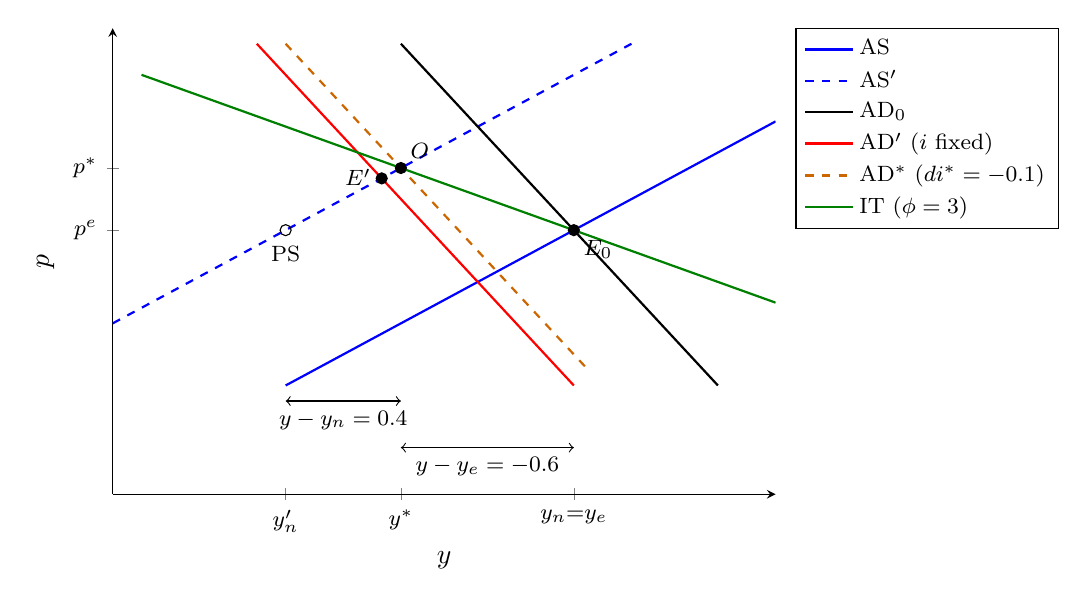
\begin{tikzpicture}
\begin{axis}[width=10cm,height=7.5cm,xmin=-1.6,xmax=0.7,ymin=-0.85,ymax=0.65,axis lines=left,xlabel={$y$},ylabel={$p$},
  xtick={-1,-0.6,0},xticklabels={$y_n'$,$y^*$,$y_n{=}y_e$},ytick={0,0.2},yticklabels={$p^e$,$p^*$},
  tick label style={font=\footnotesize},legend style={font=\footnotesize},legend pos=outer north east,legend cell align=left]
\addplot[thick,blue,domain=-1:0.7]{0.5*x};
\addplot[thick,blue,dashed,domain=-1.6:0.2]{0.5*(x+1)};
\addplot[thick,black,domain=-0.6:0.5]{-x};
\addplot[thick,red,domain=-1.1:0]{-(x+0.5)};
\addplot[thick,orange!80!black,dashed,domain=-1:0.05]{-(x+0.4)};
\addplot[thick,green!50!black,domain=-1.5:0.7]{-x/3};
\legend{AS,AS$'$,AD$_0$,AD$'$ ($i$ fixed),AD$^*$ ($di^*=-0.1$),IT ($\phi=3$)}
\addplot[only marks,mark=*] coordinates {(0,0) (-0.6667,0.1667) (-0.6,0.2)};
\addplot[only marks,mark=o] coordinates {(-1,0)};
\node[font=\footnotesize,anchor=north west] at (axis cs:0,0) {$E_0$};
\node[font=\footnotesize,anchor=east] at (axis cs:-0.67,0.17) {$E'$};
\node[font=\footnotesize,anchor=south west] at (axis cs:-0.6,0.2) {$O$};
\node[font=\footnotesize,anchor=north] at (axis cs:-1,-0.02) {PS};
\draw[<->] (axis cs:-1,-0.55) -- (axis cs:-0.6,-0.55) node[midway,below,font=\footnotesize]{$y-y_n=0.4$};
\draw[<->] (axis cs:-0.6,-0.7) -- (axis cs:0,-0.7) node[midway,below,font=\footnotesize]{$y-y_e=-0.6$};
\end{axis}
\end{tikzpicture}
\end{center}
\rubrica{\item Numbers: 1 pt. \item Graph (scored on its own): both AS, both AD, IT through $(y_e,p^e)$ with slope $-1/\phi$, $E_0$, $E'$, $O$, both gaps: 2 pts.}
\end{sol}

% -----------------------------------------------------------------------------
\questao{(10 points) \emph{Created.} Public spending rises by $\Delta>0$ in three ways: (i) temporarily, $dg=\Delta$, $d\bar g=0$; (ii) permanently,
$dg=d\bar g=\Delta$; (iii) as news only, $d\bar g=\Delta$, $dg=0$.}

\textbf{a)} (4 points) For each case: which curves move and by how much; $dy$, $dp$, $d(y-y_n)$ with $i$ fixed; and $d(y-y_e)$.
\resolespaco
\begin{sol}
\begin{notacao}
\item $y$, $p$, $\bar y$, $p^e$, $y_n$, $y_e$, $i$, $g$, $\bar g$, $\sigma>0$, $\eta>0$, $\kappa>0$, $\Omega\equiv\sigma^{-1}+\eta$: as in Question~1.
\item $\Delta>0$: the size of the spending rise. Cases (i) $dg=\Delta$, $d\bar g=0$; (ii) $dg=d\bar g=\Delta$; (iii) $dg=0$, $d\bar g=\Delta$.
\item $\phi\ge0$: weight in \eqref{LF}. $y^*$, $p^*$, $i^*$: optimal output, price and rate. $E_0$, $E'$: initial and no-policy points.
\end{notacao}
\passo{shifts}{Differentiate \eqref{YN} and \eqref{YE}:}
\begin{equation}
dy_n=dy_e=\frac{\sigma^{-1}}{\Omega}\,dg . \label{q10:dyn}
\end{equation}
So the AS shifts by $dy_n$. By \eqref{q1:dAD} and \eqref{YB}, the AD shifts by
\begin{equation}
d\bar y+dg-d\bar g=\Big(\frac{\sigma^{-1}}{\Omega}\,d\bar g\Big)+dg-d\bar g . \label{q10:ad}
\end{equation}
(i) AD $+\Delta$, AS $+\frac{\sigma^{-1}}{\Omega}\Delta$. (ii) AD $+\frac{\sigma^{-1}}{\Omega}\Delta$, AS $+\frac{\sigma^{-1}}{\Omega}\Delta$. (iii) using \eqref{q5:gb}, AD
$\big(\frac{\sigma^{-1}}{\Omega}-1\big)\Delta=-\frac{\eta}{\Omega}\Delta$, AS still. In all, \eqref{q10:dyn} gives $dy_e=dy_n$, so $d(y-y_e)=d(y-y_n)$.
\passo{(i)}{Put the shifts of (i) in \eqref{q1:M}, with $1-\frac{\sigma^{-1}}{\Omega}=\frac{\eta}{\Omega}$:}
\begin{align*}
(1+\sigma\kappa)\,d(y-y_n)&=(\Delta)-\Big(\frac{\sigma^{-1}}{\Omega}\Delta\Big)\\
&=\frac{\eta}{\Omega}\Delta .
\end{align*}
Divide by $1+\sigma\kappa$:
\begin{equation}
d(y-y_n)=\frac{\eta\Delta}{\Omega(1+\sigma\kappa)} . \label{q10:gap1}
\end{equation}
By \eqref{q1:dAS}, $dp=\kappa\,d(y-y_n)$; substitute \eqref{q10:gap1}:
\begin{align}
dp&=\kappa\Big(\frac{\eta\Delta}{\Omega(1+\sigma\kappa)}\Big)\nonumber\\
&=\frac{\kappa\eta\Delta}{\Omega(1+\sigma\kappa)} . \nonumber
\end{align}
Output is $dy=dy_n+d(y-y_n)$; use \eqref{q10:dyn} and \eqref{q10:gap1}:
\begin{align*}
dy&=\Big(\frac{\sigma^{-1}\Delta}{\Omega}\Big)+\Big(\frac{\eta\Delta}{\Omega(1+\sigma\kappa)}\Big)\\
&=\frac{(\sigma^{-1}+\kappa+\eta)\,\Delta}{\Omega(1+\sigma\kappa)}\\
&=\frac{(1+\kappa/\Omega)\,\Delta}{1+\sigma\kappa} .
\end{align*}
\passo{(ii)}{Put the shifts of (ii) in \eqref{q1:M}:}
\begin{equation}
(1+\sigma\kappa)\,d(y-y_n)=\Big(\frac{\sigma^{-1}}{\Omega}\Delta\Big)+(\Delta)-(\Delta)-\Big(\frac{\sigma^{-1}}{\Omega}\Delta\Big) . \nonumber
\end{equation}
Divide by $1+\sigma\kappa$:
\begin{equation}
d(y-y_n)=\frac{1}{1+\sigma\kappa}\Big(\frac{\sigma^{-1}}{\Omega}\Delta-\frac{\sigma^{-1}}{\Omega}\Delta\Big)=0 . \nonumber
\end{equation}
So $dp=0$ by \eqref{q1:dAS}, and $dy=dy_n=\frac{\sigma^{-1}\Delta}{\Omega}$ by \eqref{q10:dyn}.
\passo{(iii)}{Put the shifts of (iii) in \eqref{q1:M}:}
\begin{align}
(1+\sigma\kappa)\,d(y-y_n)&=\Big(\frac{\sigma^{-1}}{\Omega}\Delta\Big)-(\Delta)\nonumber\\
&=-\frac{\eta}{\Omega}\Delta . \nonumber
\end{align}
Divide by $1+\sigma\kappa$; $dy_n=0$, so output moves with the gap:
\begin{equation}
d(y-y_n)=dy=-\frac{\eta\Delta}{\Omega(1+\sigma\kappa)}<0 . \nonumber
\end{equation}
By \eqref{q1:dAS}, $dp=\kappa\,d(y-y_n)$; substitute the gap:
\begin{align}
dp&=\kappa\Big(-\frac{\eta\Delta}{\Omega(1+\sigma\kappa)}\Big)\nonumber\\
&=-\frac{\kappa\eta\Delta}{\Omega(1+\sigma\kappa)}<0 . \nonumber
\end{align}
\rubrica{\item Shifts, with $d\bar y-d\bar g=-\frac{\eta}{\Omega}d\bar g$: 1.5 pts. \item Three solutions: 2.5 pts ($-0.5$ per slip).}
\end{sol}

\textbf{b)} (3 points) Find the optimal $di^*$ in each case and show that $\phi$ does not enter. Check that (i) and (iii) add up to (ii).
\resolespaco
\begin{sol}
\begin{notacao}
\item Symbols as in (a). $X\equiv dy_e-dy_n$, as in Question 4(c).
\end{notacao}
\passo{rule}{By \eqref{q10:dyn}, $dy_n=dy_e$ in every case, so $X=0$ and \eqref{q4:ystar} gives $y^*=y_n=y_e$, $p^*=p^e$. Redo
\eqref{q4:di0}--\eqref{q4:di} with the AD shift $d\bar y+dg-d\bar g$ of \eqref{q1:dAD} in place of $d\bar y$, and set $X=0$:}
\begin{align}
di^*&=\frac{(d\bar y+dg-d\bar g)-(dy_n)}{\sigma}-\frac{(\sigma-\phi)\,\kappa\,(0)}{\sigma(1+\phi\kappa)}\nonumber\\
&=\frac{d\bar y+dg-d\bar g-dy_n}{\sigma} , \label{q10:di}
\end{align}
with no $\phi$.
\passo{cases}{Put \eqref{q10:ad} and \eqref{q10:dyn} in \eqref{q10:di}, case by case:}
\begin{align*}
\text{(i)}\quad di^*&=\frac{\Delta-\frac{\sigma^{-1}}{\Omega}\Delta}{\sigma}=\frac{\eta\Delta}{\sigma\Omega}\ \text{(raise)},\\
\text{(ii)}\quad di^*&=\frac{\frac{\sigma^{-1}}{\Omega}\Delta-\frac{\sigma^{-1}}{\Omega}\Delta}{\sigma}=0,\\
\text{(iii)}\quad di^*&=\frac{\frac{\sigma^{-1}}{\Omega}\Delta-\Delta}{\sigma}=-\frac{\eta\Delta}{\sigma\Omega}\ \text{(cut)}.
\end{align*}
Add (i) and (iii):
\begin{equation}
\frac{\eta\Delta}{\sigma\Omega}-\frac{\eta\Delta}{\sigma\Omega}=0 , \nonumber
\end{equation}
case (ii), by linearity.
\rubrica{\item Rule and $\phi$-independence: 1.5 pts. \item Three rates with signs and the sum: 1.5 pts.}
\end{sol}

\textbf{c)} (3 points) Draw the three diagrams for $\sigma=1$, $\eta=\kappa=0.5$, $\Delta=1.5$. Then, in words: what is the output multiplier when
the bank follows its optimal rule, and how does case (iii) relate to the $\bar\mu$ news of Prova 01?
\resolespaco
\begin{sol}
\begin{notacao}
\item Symbols as in (a). Values: $\sigma=1$, $\eta=\kappa=0.5$, $\Delta=1.5$. Output multiplier: $dy/\Delta$.
\end{notacao}
\passo{numbers}{The building blocks:}
\begin{align*}
\Omega&=1+0.5=1.5, & \tfrac{\sigma^{-1}}{\Omega}\Delta&=\tfrac{1.5}{1.5}=1,\\
\tfrac{\eta}{\Omega}\Delta&=\tfrac{0.75}{1.5}=0.5, & 1+\sigma\kappa&=1.5 .
\end{align*}
(i) By \eqref{q10:gap1}, $d(y-y_n)=\frac{0.5}{1.5}=\frac13$, so $dy=1+\frac13=\frac43$ and $dp=0.5\cdot\frac13=\frac16$: $E'=(\frac{4}{3},\frac16)$. The raise $\frac{\eta\Delta}{\sigma\Omega}=0.5$
moves it to $(1,0)$. (ii) $E'=(1,0)$. (iii) $dy=-\frac{0.5}{1.5}=-\frac13$, $dp=0.5\cdot(-\frac13)=-\frac16$: $E'=(-\frac13,-\frac16)$; the cut of $0.5$ brings it
back to $(0,0)$.
\begin{center}
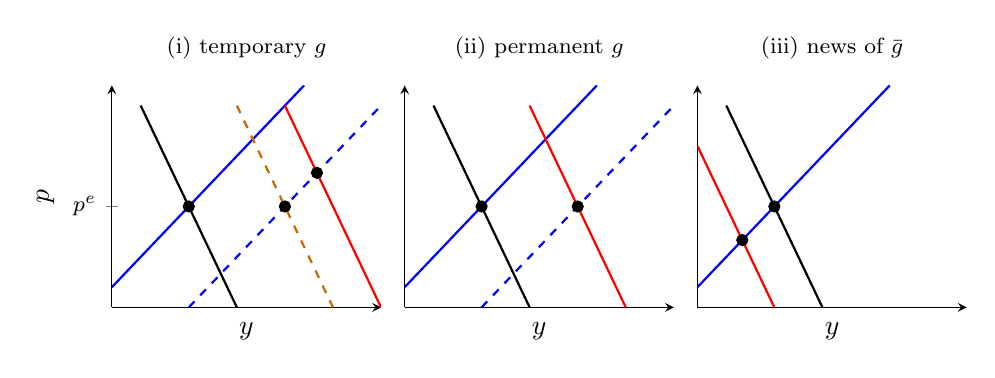
\begin{tikzpicture}
\begin{axis}[name=A,width=5cm,height=4.4cm,xmin=-0.8,xmax=2,ymin=-0.5,ymax=0.6,axis lines=left,xlabel={$y$},ylabel={$p$},
  xtick=\empty,ytick={0},yticklabels={$p^e$},title={\footnotesize (i) temporary $g$},tick label style={font=\footnotesize}]
\addplot[blue,thick,domain=-0.8:1.2]{0.5*x};\addplot[blue,thick,dashed,domain=0:2]{0.5*(x-1)};
\addplot[black,thick,domain=-0.5:0.5]{-x};\addplot[red,thick,domain=1:2]{-(x-1.5)};\addplot[orange!80!black,dashed,thick,domain=0.5:1.5]{-(x-1)};
\addplot[only marks,mark=*] coordinates {(0,0) (1.3333,0.1667) (1,0)};
\end{axis}
\begin{axis}[at={(A.east)},anchor=west,xshift=0.3cm,name=B,width=5cm,height=4.4cm,xmin=-0.8,xmax=2,ymin=-0.5,ymax=0.6,axis lines=left,
  xlabel={$y$},xtick=\empty,ytick=\empty,title={\footnotesize (ii) permanent $g$}]
\addplot[blue,thick,domain=-0.8:1.2]{0.5*x};\addplot[blue,thick,dashed,domain=0:2]{0.5*(x-1)};
\addplot[black,thick,domain=-0.5:0.5]{-x};\addplot[red,thick,domain=0.5:1.5]{-(x-1)};
\addplot[only marks,mark=*] coordinates {(0,0) (1,0)};
\end{axis}
\begin{axis}[at={(B.east)},anchor=west,xshift=0.3cm,width=5cm,height=4.4cm,xmin=-0.8,xmax=2,ymin=-0.5,ymax=0.6,axis lines=left,
  xlabel={$y$},xtick=\empty,ytick=\empty,title={\footnotesize (iii) news of $\bar g$}]
\addplot[blue,thick,domain=-0.8:1.2]{0.5*x};
\addplot[black,thick,domain=-0.5:0.5]{-x};\addplot[red,thick,domain=-0.8:0]{-(x+0.5)};
\addplot[only marks,mark=*] coordinates {(0,0) (-0.3333,-0.1667)};
\end{axis}
\end{tikzpicture}
\end{center}
{\footnotesize Blue: AS (dashed: AS$'$). Black: AD$_0$. Red: AD$'$ with $i$ fixed. Orange dashed: AD after the optimal raise in (i). In (iii) the optimal cut returns AD$'$ to AD$_0$.}
\passo{multiplier}{Under the optimal rule $y=y_n=y_e$ (part (b)), so by \eqref{q10:dyn}, in (i) and (ii), whatever the timing:}
\begin{equation}
\frac{dy}{\Delta}=\frac{\sigma^{-1}}{\Omega}=\frac{\sigma^{-1}}{\sigma^{-1}+\eta}=\frac{1}{1+\sigma\eta}<1 , \nonumber
\end{equation}
and $0$ in (iii), where $dg=0$.
The bank neutralises the demand part of fiscal policy; only its effect on capacity remains.
\passo{link to Prova 01}{(iii) is a pure AD shock from news about the long run, like $d\bar\mu>0$: AD left, AS still, prices and output fall, and
the optimal response is a cut, the same for every $\phi$.}
\refbib{Benigno (2015), \S8, Table 1, pp.~514--517; \S11, pp.~521--523.}
\rubrica{\item Graphs (scored on their own): shifts and equilibria in the three panels: 1.5 pts. \item Multiplier with the reason: 1 pt. \item Link: 0.5 pt.}
\end{sol}
